%version of 03-21-19

\chapter{NUMBERS III: OPERATIONAL NUMBER REPRESENTATIONS}
\label{ch:numerals}
\index{numerals!operational}
\index{number representations!operational}
\index{number representations}

\section{Historical and Conceptual Introduction}

Numbers are intangible idealizations.  One must endow numbers with
names before one can manipulate them and compute with them.
Historically, we have employed a broad range of mechanisms for naming
numbers.

{\ignore {\Arny I really like the idea of providing some cultural
    background to get the reader involved.}}
{\ignore {\Denis I also like the idea, may be we can shorten the Latin numbers
  and let some parts (examples) as an exercice...}}
{\ignore {\Arny Please propose what to omit.  I do want to point out the
  ``three levels'' of names/numerals: names that convey information
  only by cultural agreement; names that permit identification but no
  practical manipulation; {\em operational} names}}
\ignore{I am not sure, however, how much space to
  allocate.  For instance, I like the mention of Roman numerals and of
  the system that the Phoenicians used --- which I am familiar with
  mainly because of Hebrew --- but I am reluctant to go so far as to
  really discuss the formation rules of Roman numerals or the details
  of numeral formation in Hebrew and its kindred languages.}

\medskip

\noindent
{\it Nicknames for ``familiar'' numbers}.
%
We have endowed several numbers that are associated with concrete
entities (see the examples below) with names that do not even hint at
any aspect of the nature of the named number.  A few examples:
\begin{itemize}
\item
$\pi$: the ratio of the circumference of a circle to its diameter
\item
$e$: the base of so-called natural logarithms
\item
$\phi$: the {\it golden ratio} (one of several word-names for $\phi$)
  that can be observed in nature, e.g., in the leaf patterns of plants
  such as pineapples and cauliflower
\item
Avogadro's number: a fundamental quantity in chemistry and physics.
(This number-name indicates that not all numerical nicknames are
single letters.)
\end{itemize}
Nickname-based numerals give no information about the named number:
they do not help anyone (except the {\it cognoscenti:} the
``in-crowd'') {\em identify} the named number, and they do not help
anyone manipulate---e.g., compute with---it.  These names are valuable
only for {\em cultural} purposes, not mathematical ones.

To clarify our intended message: It is the {\em names} of these
special numbers that convey no operational information.  Each of these
is attached to valuable science and/or mathematics!  We shall expose
some of this mathematics as we discuss $e$ in the current chapter,
revisit $\pi$ and $e$ in Chapter~\ref{ch:Summation}, and revisit
$\phi$ in Chapter~\ref{ch:Recurrences}.

\medskip

\noindent
{\it Alphabet-based systems.} 
\index{alphabet-based number systems}
\index{number systems!alphabet-based}
%
Several cultures have developed systems for naming integers by using
their alphabets in some manner.  One such system that is still visible
in European cultures comprises {\it Roman numerals}.
\index{numerals!Roman} One encounters these within constrained
contexts, e.g., as hour markers on ``classical'' clocks and as
timestamps on the cornerstones of official buildings.  The numerals
are formed from a subset of the Latin alphabet:

{\small
\begin{tabular}{c|c}
{\it Letter} & {\it Numerical value} \\
\hline
I  & 1 \\
V  & 5 \\
X  & 10 \\
L  & 50
\end{tabular}
\hspace*{.5in}
\begin{tabular}{c|c}
{\it Letter} & {\it Numerical value} \\
\hline
C  & 100 \\
D  & 500 \\
M  & 1000
\end{tabular}
}

\noindent
The formation rules for Roman numerals of length exceeding $2$ are a
bit complicated, but {\em roughly}, a letter to the right of a higher
valued letter augments the value of the numeral (e.g., DCL $=650$, XVI
$=16$), while a letter to the left of a higher valued letter lowers
the value (e.g., MCM $=1900$, XLIV $=44$).

A rather different way to craft numerals from letters is observable in
the Hebrew system. \index{numerals!Hebrew} Assimilating ideas of the
ancient Egyptians, Phoenicians, and Greeks, this system assigns the
following values to the $22$ letters of the Hebrew alphabet.
\[ 1, 2, 3, 4, 5, 6, 7, 8, 9, 10,
20, 30, 40, 50, 60, 70, 80, 90, 100,
 200, 300, 400
\]
It then forms numerals as strings of single occurrences of letters, by
accumulating letters' numerical values.  Numbers that are too large to
be named via strings of single letter-instances often allow repeated
letter instances or incorporate auxiliary words, in a mixed-mode
manner similar to our writing $5000$ as ``$5$ thousand''.

\medskip

Alphabet-based systems for creating numerals are more useful than
nickname-based systems: they {\em do} allow anyone to {\em identify}
any named number. Indeed, one can (algorithmically) convert any Roman
numeral or any Hebrew numeral to a decimal numeral for the same
number.  However, any reader who is familiar with alphabet-based
systems will recognize a major drawback of such systems: It is {\em
  exceedingly difficult} to do any but the most trivial arithmetic
using such systems' numerals.  Two simple examples using Roman
numerals will make our case:
\begin{itemize}
\item
Square CC.  This is, of course, trivial using, e.g., decimal numerals:
an elementary school student can compute $200 \times 200 \ =
\ 40,000$.  But even in an early course on programming, one would not
assign the general ``multiply numbers using Roman numerals'' problem
as a first assignment.

\item
Substract MCMXCVIII from MMII.  Of course, the answer is IV, but one
would likely determine this by converting to decimal numerals
($2002-1998$).
\end{itemize}

\noindent
{\it Positional number systems.}
\index{positional number systems}
\index{number systems!positional number systems}
%
In our daily commerce, we deal almost exclusively with numerals that
are formed within a {\it base-$b$ positional number system},
\index{numerals in a base-$b$ positional number system} known also as
a {\it $b$-ary positional number system}.
\index{numerals in a $b$-ary positional number system}
The word {\it ``radix''} is often used in place of the word ``base'';
\index{numerals in a radix-$b$ positional number system}
we shall use the word ``base''.  The most common exemplars of $b$-ary
positional number systems are:

\smallskip

\begin{tabular}{llclcl}
base-$2$:  & the & $2$-ary  & or & {\em binary}      & system \\
base-$8$:  & the & $8$-ary  & or & {\em octal}       & system \\
base-$10$: & the & $10$-ary & or & {\em decimal}     & system \\
base-$12$: & the & $12$-ary & or & {\em duodecimal}  & system \\
base-$16$: & the & $16$-ary & or & {\em hexadecimal} & system
\end{tabular}

\smallskip

\noindent
Most of this chapter---specifically,
Section~\ref{sec:positional-numbers}---is devoted to studying {\em
  -ary} positional number systems in detail.

\medskip

\noindent
{\it Systems developed to ensure special properties.}
\index{number systems!formed to ensure special properties}
In Section~\ref{sec:numerals-special-properties}, we briefly describe
two families of positional systems that were invented to ensure number
representations with specific properties.  Section~\ref{sec:bijective-adic}
discusses {\em bijective number systems},
\index{positional number systems!bijective systems}
\index{positional number systems!-adic number systems}
\index{number systems!positional number systems!bijective systems}
\index{number systems!positional number systems!-adic number systems}
which are positional number systems in which distinct numerals name
distinct numbers.  This property can be significant in certain genres
of numeral-based encodings.  (Of course, -ary number systems do not
enjoy this property because of excess leading and trailing $0$s.)
Finally Section~\ref{sec:carry-free} introduces number systems that
enable {\em carry-free addition}.  This property enables the design of
``unit-time'' parallel adders of arbitrary-length numerals.

\medskip

\noindent
{\it Systems formed using special families of numbers.}
\index{number systems!based on special families of numbers}
%
In Section~\ref{sec:numerals-special-families}
The final genre of number system that we discuss in this introduction
are those based on special families of numbers, such as the binomial
coefficients and the Fibonacci numbers.  Such systems are employed
most often when the properties of the underlying family expose
particular properties of named numbers.  We discuss one such system in
Section~\ref{sec:Fibo-numbers}.


\section{Positional Number Systems}
\label{sec:positional-numbers}
\index{positional number systems}
\index{number systems!positional number systems}

We turn now to the immensely successful family of {\em operational}
numerals, the $b$-ary number systems.  Each such system is built upon
a {\em number base $b$} which is an integer $b> 1$.\footnote{In
  rather specialized contexts one may encounter number bases that are
  not positive integers.}
\index{positonal number system!number base}
The numerals in the system are strings of {\it digits} from the set
$\{0, 1, 2, \ldots, \overline{b-1}\}$, often embellished with other
symbols, such as a {\em radix point},\footnote{Using a period as the
  radix point is a US convention; in much of Europe, a comma is
  used.}~and sometimes a leading ``$+$'' or ``$-$'' to indicate,
respectively, the denoted number's positivity or negativity.

\medskip

\noindent \fbox{
\begin{minipage}{0.97\textwidth}
We employ the overline notation, ``$\overline{b-1}$'', to remind
ourselves that ``$b-1$'' is a digit \index{digit} here, not a string;
e.g., when $b = 10$ (the {\em decimal}, or, $10$-{\it ary} base),
$\overline{b-1}$ is the digit $9$.
\end{minipage}
}

\medskip

\noindent
We begin to discuss these systems with a few examples:
\begin{itemize}
\item
Most of our daily activities employ the number system usually called
{\it decimal} or {\it base-$10$}, or, unusually but also correctly,
{\it $10$-ary}.  \index{the decimal number system} 
\index{the base-$10$ number system} \index{the $10$-ary number system}
This system's digits comprise the set $\{0, 1, 2, 3, 4, 5., 6, 7, 8,
9\}$; its radix point is called a {\em decimal point}.
\index{decimal point}

\item
Because electrical and electronic circuitry are (for the most part)
built using {\it bistable} devices---e.g., switches that are either
{\em on} or {\em off}---the system most often employed when dealing
with such circuitry and its end products (say, computers) is the
{\it base}-$2$ system, which is also called {\it binary} of $2$-ary.
\index{the binary (base-2) number system}
The digits of this system comprise the set $\{0, 1\}$.  Each digit is
called a {\it bit}---a contraction of {\it binary digit}.
\index{bit: binary digit}

\item
Because of its small repertoire of digits, the binary system's
numerals are quite long---roughly $3$ times longer than decimal
numerals.  For instance, denoting the base-$b$ as a subscript to the
numeral (a common convention):
\[ 32,768_{10} \ \ = \ \ 1,000,000,000,000,000_2 \]
In order to make base-$2$e numerals easier for humans to deal with, we
usually aggregate small sequences of bits to form larger number
bases---but still powers of $2$.  Two aggregations have been
particularly popular:
  \begin{itemize}
  \item
By aggregating length-$3$ sequences of bits, one converts base-$2$
numerals to {\it base}-$8$ numerals, known also as {\it octal} or
$8$-{\it ary} numerals;
\index{the octal (base-$8$) number system} the octal digits comprise
the set $\{0, 1, 2, 3, 4, 5, 6, 7\}$.
  \item
By aggregating length-$4$ sequences of bits, one converts base-$2$
numerals to base-$16$ numerals, known also as {\it hexadecimal} or
{\it $16$-ary} numerals; \index{the hexadecimal (base-$16$) number system} 
the hexadecimal digits comprise the set 
\[ \{0, 1, 2, 3, 4, 5, 6, 7, 8, 9, \overline{10}, \overline{11},
\overline{12}, \overline{13}, \overline{14}, \overline{15}\}.
\]
{\it Note:} We have written the hexadecimal digits in decimal, to make
them easy to read, but we have placed overlines above the
$2$-decimal-digit numerals ``$10$'', ``$11$'', ``$12$'', ``$13$'',
``$14$'', and ``$15$'' as a reminder that each represents a single
hexadecimal digit, not a $2$-digit numeral.
  \end{itemize}
The success of these aggregations is attested to by the following
equation chain:
\[ 32,768_{10} \ \ = \ \ 1,000,000,000,000,000_2 \ \ = \ \
100,000_8 \ \ = \ \ 8,000_{16}
\]
\end{itemize}

\subsection{$b$-ary Number Systems}
\label{sec:b-ary-systems}

The {\it $b$-ary} number systems are by far the most commonly used
positional number systems.  The names of the different instances of
the system---each formed by choosing a specific number base
$b$---derive from the {\em Latin} name of the base number.
Regrettably, from a denotational point of view, the systems associated
with certain bases end with the suffix {\em -ary} (as in ``binary'')
while those associated with other bases end with the suffix {\em -al}
(as in ``decimal'').  The following table codifies the multiple names
of the systems associated with the most commonly used bases (for
mathematicians, scientists, and engineers).

\smallskip

\begin{tabular}{|c|l|l|}
\hline
{\bf Base} & \multicolumn{2}{c}{\bf {\em -ary} System Names}  \\
\hline
$2$   & binary     & $2$-ary  \\
\hline 
$4$   & quaternary & $4$-ary  \\
\hline
$8$    & octal & $8$-ary \\
\hline
$10$   & decimal & $10$-ary  \\
\hline
$12$    & duodecimal & $12$-ary  \\
\hline
$16$     & hexadecimal & $16$-ary \\
\hline
\end{tabular}

\bigskip

\index{positional number system!forming base-$b$ numeral}
\noindent {\bf The formation rules for $b$-ary numerals}.
As we turn to the {\it formation rules} for $b$-ary numerals, we want
to emphasize that these rules build in an essential way on the ideas
relating to summing {\em geometric summations}.  This is, therefore, a
good time to review Section~\ref{sec:geometric-sums}.

\medskip

%{\Denis the following should be put before in 4.5.2}

\index{base-$b$ numeral}
\index{positional number system!base-$b$ numeral}
\index{$b$-ary numeral}
\index{positional number system!$b$-ary numeral}
\noindent
A $b$-ary numeral is a string having three segments.
\begin{enumerate}
\item
The numeral begins with its {\em integer part},
\index{positional number system!base-$b$ numeral!integer part}
\index{base-$b$ numeral!integer part}
which is a {\em finite} string of base-$b$ digits, i.e., digits from
the set \index{$B_b$: $b$-ary digits}
\begin{equation}
\label{eq:b-ary-digits}
B_b \ \eqdef \ \{0, 1, 2, \ldots, \overline{b-1}\}
\end{equation}
(Recall that ``$\overline{b-1}$'' represents the integer $b-1$ as a
single digit.)  \index{$\overline{b-1}$: $b-1$ as a single digit}
We denote the integer-part string as: $\alpha_n \alpha_{n-1} \cdots
\alpha_1 \alpha_0$.

\item
The numeral continues with a single occurrence of the {\it
  radix point},
\index{positional number system!radix point}
\index{positional number system!base-$b$ numeral!radix point}
\index{base-$b$ numeral!radix point}
which is denoted ``$.$'' in the U.S.~and ``,'' in many other countries. 

\item
The numeral ends with its {\em fractional part},
\index{positional number system!fractional part of a numeral}
\index{positional number system!base-$b$ numeral!fractional part}
\index{base-$b$ numeral!fractional part}
which is a string---{\em finite or infinite}---of base-$b$ digits We
denote the fractional-part string as: $\beta_0 \beta_1 \beta_2
\cdots$.
\end{enumerate}
Our completed numeral now has the form
\begin{equation}
\label{eq:real-numeral}
\alpha_n \alpha_{n-1} \cdots \alpha_1 \alpha_0
\ . \ \beta_0 \beta_1 \beta_2 \cdots
\end{equation}

\noindent
This numeral has the {\it numerical value}\footnote{The notation
  ``$\mbox{\sc val}_{b}(x)$'' in (\ref{eq:real-numeral-number})
  denotes an operator that produces the {\em numerical value} of the
  base-$b$ numeral $x$.}
\begin{equation}
\label{eq:real-numeral-number}
\mbox{\sc val}_{b}(\alpha_n \alpha_{n-1} \cdots \alpha_1 \alpha_0                  
\ . \ \beta_0 \beta_1 \beta_2 \cdots)
\ \ \eqdef \ \
\sum_{i=0}^n \alpha_i \cdot b^i
\ + \ \sum_{j\geq 0} \beta_j \cdot b^{-j}.
\end{equation}
\index{positional number system!numerical value of base-$b$ numeral}
\index{base-$b$ numeral!numerical value}
\index{positional number system!base-$b$ numeral!numerical value}
For emphasis, we review:
\index{positional number system!numerical value of integer part}
\begin{itemize}
\item
The numerical value of the integer part of the numeral in
(\ref{eq:real-numeral}) is:
\[
\mbox{\sc val}_{b}(\alpha_n \alpha_{n-1}\cdots \alpha_1 \alpha_0)
\ \ = \ \
\sum_{i=0}^n \alpha_i \cdot b^i
\]
\item
The numerical value of the fractional part of the numeral in
(\ref{eq:real-numeral}) is:
\index{positional number system!numerical value of fractional part}
\[
\mbox{\sc val}_{b}(. \beta_0 \beta_1 \beta_2 \cdots)
\ \ = \ \
\sum_{j\geq 0} \beta_j \cdot b^{-j}
\]
\item
By prepending a ``minus sign'', or, ``negative sign'' ($-$) to a
numeral or a number, one renders the thus-embellished entity as
negative.
\end{itemize}

Note that {\em two types of sequences of $0$s do not affect the value
  of the number represented by a $b$ary numeral:}
\begin{itemize}
\item
an {\em initial} sequence of $0$s that reside to the {\em left} of the
radix point and of all non-$0$ digits;
\item
a {\em terminal} sequence of $0$s that reside to the {\em right} of
the radix point and of all non-$0$ digits.
\end{itemize}
One consequence of this fact is that we lose no generality by
insisting that every numeral have the following {\em normal form:}
\index{positional number system!numeral!normal form}
\index{normal form for for numeral in a positional number system}

\smallskip

\hspace*{.15in}
\begin{tabular}{l}
-- it begins with a finite sequence of digits, \\
-- it then has one occurrence of the radix point, \\
-- it ends with an infinite sequence of digits
\end{tabular}

\bigskip

We finish this section with an important consequence of the definition
of real numbers in Section~\ref{sec:define-Reals}, in terms of the
summations in (\ref{eq:real-defn}).

\begin{prop}
\label{thm:define-Reals-via-numerals}
A number $n$ is real, i.e., belongs to the set $\R$, if, and only if
it is the numerical value of a numeral of the form
(\ref{eq:real-numeral}).
\end{prop}

{\Arny A good exercise ?}

\subsection{$\oplus$ Positional Number Systems with Special Properties}
\label{sec:numerals-special-properties}

Among the many ``nonstandard'' positional number systems that have
been invented because of some special characteristic(s), we have
selected two, chosen because of their importance to some scientific
endeavor.

\subsubsection{A {\em bijective} number system}
\label{sec:bijective-adic}
\index{positional number system!bijective}

This section introduces a positional number system in which distinct
numerals name distinct numbers.  Of course, $b$-ary systems do not
enjoy this property because of the value neutrality of leading $0$s
for integer numerals and trailing $0$s for fractional numerals.  The
systems are often termed {\it bijective} because their unique numerals
for integers arise from a bijection between the integer numerals and
the set $\N^+$ of positive integers.  {\em The price that these
  systems pay for their bijectiveness is that they cannot represent
  the number $0$; they can represent all other integers.}  Each
bijective base-$b$ system is sometimes called the {\it $b$-adic number
  system}. \index{positional number system!$b$-adic} One also finds
some -adic number systems being named using Greek-inspired names for
the base $b$, in imitation of the Latin-inspired names of -ary
systems.  Most commonly one encounters the base-$2$ {\it dyadic}
\index{positional number system!dyadic: base-$2$}
\index{dyadic (base-$2$) number system} system as the -adic analogue
of the binary system.

For any number base $b > 1$, the base-$b$ bijective systems' numerals
are formed in exactly the same way as are the numerals of the $b$-ary
number system---see (\ref{eq:real-numeral-number})---but the bijective
systems' numerals are formed using the digit-set $B'_b \ = \ \{1, 2,
\ldots, b\}$, rather than the $b$-ary set $B_b$ of
(\ref{eq:b-ary-digits}).  In order to lend the reader some intuition,
we display the dyadic numerals that have one or two digits together
with their numerical values.

\smallskip

\begin{tabular}{|lc|ll|}
\hline
\multicolumn{2}{c}{\bf Dyadic Numeral} & \multicolumn{2}{c}{\bf Numerical Value} \\
\hline
$x=$ & $1$  & {\sc dyadic-val}$(x) =$ & $1$ \\
     & $2$  &                         & $2$ \\
     & $11$ &                         & $2 + 1 = 3$ \\
     & $12$ &                         & $2 + 2 = 4$ \\
     & $21$ &                         & $4 + 1 = 5$ \\
     & $22$ &                         & $4 + 2 = 6$ \\
\hline
\end{tabular}

\medskip
\noindent
The preceding table indicates how the numerical values of dyadic
numerals track the lexicographic order of the numerals.

\bigskip

Formally verifying the bijectiveness of $b$-adic number systems is a
valuable exercise in manipulating numerals.  The first appearance of
bijective number systems was in \cite{Foster47}, where the base-$10$
system is introduced and shown to be bijective.  A proof of
bijectiveness for arbitrary $b$-adic systems appears in
\cite{Smullyan61}, where the term {\em $b$-adic} is introduced.  The
motivating application in \cite{Smullyan61} was to the allied fields
of Mathematical Logic and Computation Theory: Encoded versions of a
program's computations play a central role in these theories.  While
crafting the required encodings using strings of symbols accomplished
many of the goals of the theories, the overarching reach of the
theories was fully appreciated only when mathematical logician Kurt
G\"{o}del \index{G\"{o}del, Kurt} showed, in 1931, that the encodings
could be achieved using integers and simple arithmetic
operations---see the discussions of {\it G\"{o}del numbers}
\index{G\"{o}del numbers} in the primary sources
\cite{Goedel31,Turing36} or texts such as \cite{Rosenberg12}.  The
introduction in \cite{Smullyan61} of -adic number systems to replace
the traditional -ary systems significantly simplified certain of the
theories' central proofs, because of the -adic systems' bijectiveness.

We turn now to a result that asserts the bijectiveness of -adic number
systems.  We provide a proof only for the case $b = 2$: this case
provides all of the ideas necessary for the general result.

\begin{prop}
\label{thm:adic-bijective}
Distinct $b$-adic numerals name distinct positive numbers.
\end{prop}

\begin{proof}[For dyadic integers]
We provide a proof only for dyadic, i.e., base $b=2$, integers.  This
will expose the basic ideas of a complete proof, with minimal
notation.  We begin by exposing the largest and smallest integers that
admit a $d$-digit dyadic numeral.

\begin{lemma}
\label{lem:big-small-dyadic}
The {\em smallest} integer representable by a $d$-digit dyadic
numeral is 
\[ \mbox{\sc min-integer}_d \ = \ 2^d + 2^{d-1} + \cdots + 1 \ = \ 2^{d+1} - 1
\]
The {\em largest} integer representable by a $d$-digit dyadic
numeral is
\[ \mbox{\sc max-integer}_d \ = \
2 \times (2^d + 2^{d-1} + \cdots + 1) \ = \ 2^{d+2} - 2
\]
\end{lemma}

\begin{proof}[Lemma]
By definition,
\begin{itemize}
\item
The smallest $d$-digit dyadic numeral is $11 \cdots 1$ ($d$ digits).
Its value is:
\[ \mbox{\sc dyadic-val}_2(11 \cdots 1)
 \ = \ 2^d + 2^{d-1} + \cdots + 1 \ = \ 2^{d+1} - 1 \]
\item
The {\em largest} $d$-digit dyadic numeral is 
$22 \cdots 2$ ($d$ digits).  Its value is:
\[ \mbox{\sc dyadic-val}_2(22 \cdots 2)
\ = \ 2 \times (2^d + 2^{d-1} + \cdots + 1) \ = \ 2^{d+2} - 2 \]
\end{itemize}
We derive the values of both extremal integers by invoking the
summation techniques in Section~\ref{sec:geometric-sums}.
\qed-Lemma
\end{proof}

\bigskip

We are now ready to prove the proposition.  To this end, let us be
given distinct dyadic numerals,
\[
x \ = \ \gamma_r \gamma_{r-1} \cdots \gamma_1
 \ \ \ \ \ \mbox{ and } \ \ \ \ \
y \ = \ \delta_s \delta_{s-1} \cdots \delta_1
\]

{\bf (a)} Say first that $r \neq s$.  With no loss of generality, say
that $r = s +c$ for some $c \geq 1$.  In this case, we have, by
Lemma~\ref{lem:big-small-dyadic}:
\[ \mbox{\sc dyadic-val}(x) \ \geq \ 2^{r+1} - 1 \ = \ 2^{s+c+1} -1 \]
while
\[ \mbox{\sc dyadic-val}(y) \ \leq \ 2^{s+2} - 2 \]
It follows, therefore, that
\[ \mbox{\sc dyadic-val}(x) \ \geq \ \mbox{\sc dyadic-val}(y) \ + \ 1 \]
In particular, numerals $x$ and $y$ behave in consistency with the
proposition.

{\bf (b)} The alternative to assumption (a) is that $r = s$.  Because
$x$ and $y$ are distinct numerals, there must be a largest index $m
\leq r$ such that $\gamma_m \neq \delta_m$; say, with no loss of
generality, that $\gamma_m = \delta_m + c$ for some base-$b$ dyadic
digit $c$.  We can, therefore, rewrite numeral $y$ as
\[ y \ = \ \gamma_r \cdots \gamma_{m+1} \delta_m \delta_{m-1} \cdots \delta_1
\]
Invoking Lemma~\ref{lem:big-small-dyadic}, we can infer the following
bounds on the difference between $\mbox{\sc dyadic-val}(x)$ and
$\mbox{\sc dyadic-val}(y)$.

\bigskip

$\mbox{\sc dyadic-val}(x) \ - \ \mbox{\sc dyadic-val}(y)$
\begin{eqnarray*}
  & =  &
2^m \cdot (\gamma_m - \delta_m) \ + \ 2^{m-1} \cdot (\gamma_{m-1} -
\delta_{m-1}) \ + \cdots + \  2 \cdot (\gamma_1 - \delta_1) \\
  & \geq &
2^m \cdot (\gamma_m - \delta_m) \ - \ \left( 2^{m-1} + 2^{m-2} +
\cdots + 1 \right) \\
  & = &
2^m \cdot (\gamma_m - \delta_m)\ - \ \left( 2^m -1 \right) \\
  & = &
2^m \cdot (c-1) +1 \\
  & \geq & 1
\end{eqnarray*}
Once again, numerals $x$ and $y$ behave in consistency with the
proposition.  The result follows.
\qed
\end{proof}


\subsubsection{Signed-digit systems: carry-free addition}
\label{sec:carry-free}

Say that you have a box that contains a {\it counter}.  There are two
buttons on top of the box: one {\em red} and one {\em green}.  Each
time the green button is pushed, the counter increments---i.e., adds
$+1$ to---its tally; each time the red button is pushed, the counter
decrements---i.e., adds $11$ to---its tally.  Now, in order for the
tally on the counter to {\em always be correct}, you must insert
delays between button-pushes: you must always wait until the
electronic circuitry inside the box settles into a stable
configuration with all necessary carries and borrows up to date.  Now,
if the electronic circuitry that implements the counter was designed
to mimic the binary representation of the number---in technical
jargon, \index{carry-ripple adder} the counter implements a {\it
  carry-ripple adder}; see \cite{Hwang79} for details---then, you
observe the following.  While you keep pushing only the green
(increment) button, you do not feel that the delays between
button-pushes are onerous: As we noted in
Section~\ref{sec:sample-proofs}.A:
\begin{itemize}
\item
Roughly half the time, you have no enforced delays between successive
button-pushes: the update of the tally engenders no carry.
\item
Roughly one-quarter of the time, you have a miniscule delay: the
update engenders a carry of only one place.
\item
Roughly one-eighth of the time, you have a slightly longer delay: the
update engenders a carry of two places.
\item
\ldots Continuing this progression: For each integer $k$ roughly the
fraction $2^{-k}$ of the button-pushes engender a delay commensurate
with a carry of $k-1$ places.
\end{itemize}
Stated differently, the {\em average} delay you must suffer is bounded
by the time required for a $2$-place carry.  In fact, you can even
improve on the described pattern of delays, by using more
sophisticated circuitry for your counter's adder.  If you replace the
carry-ripple adder by a {\it carry-lookahead adder}---see
\cite{Hwang79} for details---you can thereby reduce the aggregate
number of carries engendered by the first $n$ button-pushes from the
$\Theta(n^2)$ carries of the carry-ripple adder to $O(n \log n)$
carries for a carry-lookahead adder.

But, the picture changes markedly as soon as you (or an opponent)
starts using the red button as well as the green one.  If you wait
until the counter has tallied some number of green-button pushes of
the form $2^k$, hence contains the binary numeral $100 \cdots 00$ with
$k$ $0$s, then a push of the red button engenders a delay of $k$
carry-units---and a subsequent push of the green button incurs the
same delay!  In fact, if you (and your opponent) begin to toggle the
two buttons---one red push, then one green push, then one red push,
then one green push, \ldots---then you incur a delay of $k$
carry-units with each successive button-push.  If you do this for long
enough, then your {\em average} delay starts growing toward $k$
carry-units.

If (the risk of) these long delays is more than you want to deal with,
then you can employ mathematical and electronic technology to replace
your counter's adder with one that (almost) eliminates these delays
completely.  The ``silver bullet'' resides in using a {\em
  signed-digit} (positional) number representation
\index{signed-digit number representation}
\index{positional number representation!signed-digit representation}
to design a counter that implements {\it carry-free addition}.
\index{carry-free addition} By changing the form of numerals, one can
design adders whose constituent digit-adders can operate in parallel.
While these digit-adders are roughly twice as complex as those of the
more familiar carry-ripple adders, they do guarantee bounded---i.e.,
$O(1)$---delay between button-pushes, no matter how long you keep
pushing a button or which one you choose to push.

The signed-digit number systems that we discuss\footnote{There are
  many such systems and many places to learn about them; see, e.g.,
  the encyclopedic work \cite{Knuth69} on ``seminumerical algorithms''
  and the comprehensive text \cite{Hwang79} on computer
  arithmetic.}~are positional systems of the same genre as -ary
systems: Their numerals are also evaluated by the {\sc val} function
of (\ref{eq:real-numeral-number}).  These systems achieve their
buffered carries via augmented digit-sets that include {\em negative}
digits as well as positive ones.  The base-$b$ (or, {\it radix}-$b$)
redundant number system \index{base-$b$ signed-digit number system}
\index{radix-$b$ signed-digit number system} has the following set of
digits.\footnote{($a$) Recall that the overline notation, as in
  ``$\overline{b-2}$'' is to indicate that we are referring to a
  single digit.  ($b$) We add parentheses when we describe
  $\widehat{B}_b$ to enhance legibility.}
\[ \widehat{B}_b \ = \ \{(-\overline{b-1}), (-\overline{b-2}), \ldots,
(-1), 0 , 1, \ldots, \overline{b-2}, \overline{b-1}\}
\]
For technical reasons, the simple carry-free adder that we describe
requires that the number base $b$ be n smaller than $3$.  For the
smallest relevant base, $b=3$, one can use the digit-set
$\widehat{B}_3 \ = \ \{ (-2), (-1), 0, 1, 2\}$ (parentheses added to
enhance legibility).  The ``redundancy'' in this system is witnessed
by the fact that the number $1$ is the numerical value of {\em every}
numeral of the form
\[ 1 \ (-2) \ (-2) \ \cdots \ (-2) \ (-2), \]
because the $d$-digit instance of these numerals has numerical value

\smallskip

$\displaystyle \mbox{\sc val}_3 \big( 1 \ (-2) \ (-2) \ \cdots \ (-2) \ (-2) \big)$

\smallskip

\hspace*{.25in}$= \ 3^{d-1} \ - \ 2 \cdot \big(3^{d-2} \ + \ 3^{d-3}
\ + \cdots + \ 3 \ + \ 1 \big)$

\hspace*{.25in}$= \ 1$

\bigskip

We now provide a schematic description of ($a$) a carry-ripple adder
and ($b$) a carry-free adder adding the $b$-ary integer-specifying
numerals
\[ x_n x_{n-1} \cdots x_1 x_0 \ \ \ \mbox{ and } \ \ \ 
y_n y_{n-1} \cdots y_1 y_0
\]
In both descriptions, we describe the function of the $i$th
digit-adder, emphasizing the information that it receives from the
$(i-1)$th digit-adder and the information that it transmits to the
$(i+1)$th digit-adder.  Of course, this information is at the heart of
the issue of carries or no-carries.

A detailed description of both genres of adders---including both
operational and implementational matters---can be found in sources
such as \cite{Hwang79}.

\begin{figure}[hbt]
\[
\begin{array}{|lcccr|}
\hline
 & & x_i \ \ \ y_i & & \\
 & & \downarrow \ \ \ \downarrow & & \\
c_{i+1} \ = \ \big( (x_i + y_i + c_i) \ominus \bar{b} \big)
 & & \longleftarrow \ \fbox{$x_i + y_i + c_i$} \ \longleftarrow & &  c_i 
  \\
 & & \downarrow & &
  \\
 & & z_i \ = \ \min \big( \bar{b}, \ x_i + y_i + c_i \big)  & & 
  \\
\hline
\end{array}
\]
\caption{Digit $i$ of a $b$-ary carry-ripple adder.  The input digits
  $x_i$ and $y_i$ are summed with the in-carry $c_i$.  If the sum can
  be represented by a single $b$-ary digit, then it is the output from
  this digit-adder, and the out-carry $c_{i+1}$ is set to $0$.  If the
  sum is too big, then the maximum $b$-ary digit $\bar{b}$ is the
  output from this digit-adder, and the out-carry $c_{i+1}$ is set to
  the portion of the sum that exceeds $\bar{b}$.}
\label{fig:carry-ripple-digit}
\end{figure}

\bigskip

\noindent {\it A Carry-ripple adder}. \index{carry-ripple adder}
See Fig.~\ref{fig:carry-ripple-digit}.
\begin{itemize}
\item
All digits---input digits $x_i$ and $y_i$, and carry digit $c_i$ (for
$i>0$) come from $B_b = \{ 0, 1, \ldots, \bar{b}\}$; $c_0 = 0$.
\item
Addition is a {\em single-pass} process.  For each digit-index $i$:
  \begin{itemize}
  \item
Digit-adder $i$ admits inputs $x_i$ and $y_i$ (from the ``outside'')
and carry-in $c_i$: When $i=0$, $c_0 = 0$ by convention; for all other
indices $i$, $c_i$ is the carry-in from digit-adder $i-1$.
  \item
The $i$th sum-digit, $z_i$, and the carry-out, $c_{i+1}$, are
evaluated as follows.
\[
\begin{array}{ccccccc}
 z_i    & = &  \min \big( \bar{b}, \ x_i + y_i + c_i \big) & & & & \\
c_{i+1} & = &  (x_i + y_i + c_i) \ominus \bar{b} &
\mbox{ where } &
m \ \ominus \ n &  \eqdef & \left\{
{\displaystyle
\begin{array}{cl}
m-n & \mbox{ if } \ \ m \geq n \\
0   & \mbox{ if } \ \ m \leq n
\end{array}
} \right.
\end{array}
\]
  \end{itemize}
\end{itemize}

\bigskip


\begin{figure}[hbt]
\[
\begin{array}{|llcccr|}
\hline
 & & & x_i \ \ \ y_i & & \\
 & & & \downarrow \ \ \ \downarrow  & & \\
\mbox{\bf stage $1$:   } & t_{i+1} & \longleftarrow &
\fbox{
\begin{tabular}{c}
Compute \\
$\tau_i$ \ \ and \ \ $t_{i+1}$ \\
via the relation \\
$b \cdot t_{i+1} + \tau_i \ = \ x_i + y_i$
\end{tabular}
} & & \\
  & & & \downarrow & & \\  
  & & & \tau_i & & \\
  & & & \downarrow & & \\ 
\mbox{\bf stage $2$:   } & & &  \fbox{Compute $\tau_i + t_i$} & \longleftarrow & t_i 
  \\
  & & & \downarrow & &
  \\
  & & & z_i & &
  \\
\hline
\end{array}
\]
\caption{Digit-adder $i$ of a $(b > 2)$-ary carry-free adder.  The
  outgoing {\it transfer digit} $t_{i+1}$ and the {\it tentative sum}
  $\tau_i$ are computed from the input digits $x_i$ and $y_i$, using
  the relation specified in the upper box.  These results are
  transmitted, respectively, to stage $1$ of digit-adder $i+1$ and
  stage $2$ of the current digit-adder $i$.}
\label{fig:carry-free-digit}
\end{figure}

\noindent {\it A Carry-free adder}. \index{carry-free adder}
See Fig.~\ref{fig:carry-free-digit}.
\begin{itemize}
\item
This simple carry-free adder operates in {\em two-stages}.  It
operates on base-$b$ numerals but requires $b > 2$ (for technical
reasons).
\item
There is no ``carry digit''.  In its place, there is a {\it transfer
  digit} $t_i \in \{-1, 0, 1\}$ 
\index{carry-free adder!transfer digit} which is generated in stage
$1$ of the adder and consumed in stage $2$.
\item
In addition to transfer digits, there are {\it tentative sum} digits
$\tau_i$, \index{carry-free adder!tentative-sum digits} 
which are also generated in stage $1$ and consumed in stage $2$.
\end{itemize}
\begin{enumerate}
\item
Stage $1$ of the adder
\begin{enumerate}
\item
computes {\it transfer digit} $t_{i+1} \in \{-1, 0 , 1\}$ and {\it
  tentative-sum digit} $\tau_i$ via the equation
\[ b \cdot t_{i+1} + \tau_i \ = \ x_i + y_i \]
\item
transmits $t_{i+1}$ to digit-adder $i+1$
\item
transmits $\tau_i$ to stage $2$.
\end{enumerate}
\item
Stage $2$ of the adder computes the $i$th output digit $z_i$ via by
adding $\tau_i$ to $t_i$ (which came from digit-adder $i-1$).
\end{enumerate}
The important fact to note is that this adder does not have a chain of
propagated carries!  Digit-adder $i$ computes transfer digit
$t_{i+1}$---which is the only information that it transmits to
digit-adder $i+1$---based only on the $i$th input digits $x_i$ and
$y_i$.  Consequently: {\em All of the adder's digit-adders can operate
  in parallel!}



\section{$\oplus$ A System Based on the Fibonacci Numbers}
\label{sec:numerals-special-families}
\label{sec:Fibo-numbers}

**HERE

%{\Denis I suggest to add a section on numbering systems (we already
%spoke about binary system, I would like to add a section on Fibonacci
%numbering system), I put it in the following, but may be we will have
%to put somewhere else, or as an exercice?}

In a variety of application areas, the special properties of certain
families of numbers can be exploited if one uses the numbers in the
family to devise representations of all integers.  We illustrate this
fact while using the Fibonacci numbers---see
Section~\ref{sec:Fibonacci}---as our basis family.

\noindent
We shall repeatedly find the following nonstandard notation useful:

For integers $m$ and $n$, we write $[m \gg n]$ to mean that $m \geq
n+2$.

\medskip


We will first prove the \textit{Zeckendorf's theorem} which states
that every positive integer $n$ has a unique representation of the
form:  **CITATION**

$n = F(k_1) + F(k_2) + ... + F(k_r)$ where $k_1 \gg k_2 \gg ... \gg k_r$ and $k_r \geq 2$.

Here, we assume that the Fibonacci sequence starts at index $1$ and not $0$,
moreover, the decompositions will never consider $F(1)$ (since $F(1)=F(2$)). 
For instance, the representation of $12345$ turns out to be:

$12345 = 10946 + 987 + 377 + 34 + 1 = F(21) + F(16) + F(14) + F(9) + F(2)$
\bigskip

Figure~\ref{zeckendorf} shows the decomposition of the first 26 integers written in this system. 
\begin{figure}[h]
\begin{center}
%\includegraphics[width=0.4\textwidth]{../FIGmaths/zeckendorf_representations.png}
        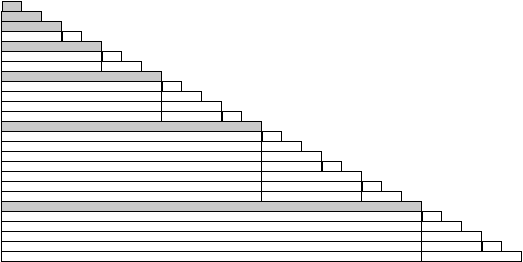
\includegraphics[scale=0.6]{FiguresArithmetic/Zeckendorf}
        \caption{The first integers (on the Y-axis) broken down into the Zeckendorf representation.
        The shaded rows corresponds to pure Fibonacci numbers.}
\label{zeckendorf}
\end{center}
\end{figure}

\noindent \textbf{Proof of Zeckendorf's Theorem}

The proof is done by induction on $n$ for proving simultaneously both construction and uniqueness.

\begin{itemize}
\item
The basis is true since the decomposition is obviously unique for $n=2$ (and also for $n=3$). 
Notice that for $n=4$, we have $4 = 3 + 1 = F(4) + F(2)$. 

\item
Assume for the induction step that any integer strictly lower than $F(k)$ can be decomposed uniquely as the sum of non-consecutive Fibonacci numbers.
We will prove as a consequence that an integer $n$ in the next interval between two consecutive Fibonacci numbers $F(k) \leq n < F(k+1)$ may be decomposed. 

If $n=F(k)$ is a Fibonacci number, the decomposition is reduced to $F(k)$.

Moreover, it is not difficult to check that it is unique.

%by using Property~\ref{prop:FiboSum}:
%$F(k) = 2+ \sum_{i=1}^{k-2} F(i)$ (the 2 comes from the shift of the starting element of the sequence...).

\medskip

If $n \neq F(k)$ write $n = F(k) + N$.

As $N$ is strictly lower than $F(k)$, we apply the recurrence hypothesis to decompose it into non-consecutive Fibonacci numbers:

$n = F(k) + F(k_1) + F(k_2) + \cdots + F(r)$ where $k_2 \gg ... \gg k_r \geq 2$. 

The last point to verify is that $F(k)$ and $F(k_1)$ are not consecutive ($F(k) \gg F(k_1)$), which is done by contradiction:

Assuming $k$ and $k_1$ are consecutive ($k_1=k-1$) leads to $n = F(k+1) + F(k_2) + \cdots + F(r)$
which contradicts $n < F(k+1)$.
\end{itemize}

Any unique system of representation is a numbering system.

The previous theorem ensures that any non-negative integer can be written
as a sequence of bits $b_i$, in other words,

$n = (b_mb_{m-1}...b_2)_F$ iff $n = \Sigma_{k=2}^m b_k F(k)$.

Note: we wrote here the representation of $n$ in the Fibonacci numbering system using parenthesis in order to avoid confusions 
on the indices.

Let us compare this system to the binary representation.
For instance, the Fibonacci representation of $12345$ is $100001010000100000010_F$
while  $12345 = 2^{13} + 2^{12} + 2^{5} + 2^{4} + 2^{3} + 2^{0} = 1100000111001_2$.
The binary representation is more compact. 
\bigskip

The decomposition in the Fibonacci basis of the first integers (starting from $1 = 00001_F$) is as follows:

 $2 = 0010_2 = F(3) = 00010_F$
 
 $3 = 0011_2 = F(4) = 00100_F$
  
 $4 = 100_2 = 3+1 = 00101_F$
 
 $5 = 101_2 = F(5) = 01000_F$
 
 $6 = 110_2 = 5+1 = 01001_F$
 
 $7 = 111_2 = 5+2 = 01010_F$
 
 $8 = 1000_2 = F(6) = 10000_F$
 
 $9 = 1001_2 = 10001_F$
 
 $10 = 1010_2 = 10010_F$
 
 $11 = 1011_2 = 10100_F$
 
 $12 = 1100_2 = 10101_F$
 
 $13 = 1101_2 = F(7) = 100000_F$
 
 ...
 
There is no consecutive digits equal to $1$ in such representations.


\section{Recognizing Integers and  Rationals from Their $b$-ary Numerals}
\label{sec:special-numerals-N-Q}

We have provided an adequate, albeit inelegant, characterization of
the real numbers: a number $r$ is real if, and only if, it can be
represented by an infinite-length numeral in a positional number
system.  Because every rational number---hence, also, every
integer---is also a real number, every rational number and every
integer can also be written as a $b$-ary numeral, in the form
(\ref{eq:real-numeral}).  For rational numbers and integers, we can
make much stronger statements about the forms of their positional
numerals.


\subsection{Positional numerals for integers}
\label{sec:special-numerals-N}

The following result slightly alters the usual way that we write
numerals for integers, in order to render explicit the familial
relationship between reals and integers.

\begin{prop}
\label{thm:integer-real}
A real number is an integer if, and only if, it can be represented by
a {\em finite-length} numeral all of whose nonzero digits are to the
left of the radix point.
\index{number!integer!as a real with a finite numeral}
\end{prop}

\begin{proof}
The result follows from definition (\ref{eq:real-numeral-number}).  In
the indicated form, if any $\beta_i$ is nonzero, then the numerical
value of the numeral is non-integral.  To wit, digit $\beta_i$
witnesses that the numeral has a nonzero fractional part, hence is not
an integer.  \qed
\end{proof}

We can go beyond the simple statement of
Proposition~\ref{thm:integer-real} and develop an efficient algorithm
that computes the base-$b$ numeral for an integer $n$ via a series of
integer divisions.

\bigskip

\noindent {\it To compute a (finite) base-$b$ numeral for integer $n$.}
\index{number!integer!computing an integer's finite numeral}
%
If we ignore the radix point and all of the $0$s to the right of it in
the base-$b$ numerals given by (\ref{eq:real-numeral}), then we see
that the base-$b$ numeral $a_d a_{d-1} \cdots a_1 a_0$ for an integer
$n$ is a polynomial

$P(x) \ \ = \ \ a_0 \ + \ a_1 x \ + \ a_2 x^2 \ + \cdots + \ a_{d-1}
x^{d-1} \ + \ a_d x^d$

\noindent
evaluated at the point $x=b$:

$\mbox{\sc val}_{b}(x) \ \ = \ \ a_d b^d \ + \ a_{d-1} b^{d-1} \ +
\cdots + \ a_1 b \ + \ a_0$.

\noindent
It appears at first glance that $\Theta(d^2)$ multiplications are
needed to evaluate the preceding degree-$d$ univariate
polynomial---which woud not give us a very efficient procedure for
producing a numeral for $n$.  However, we can develop an efficient,
$O(d)$-multiplication, procedure by adapting a method of rewriting
univariate polynomials which is known variously as {\it Horner's rule}
or {\it Horner's scheme} \cite{Horner}. \index{Horner's rule}
\index{Horner's scheme} By describing Horner's rule on a degree-$3$
polynomial, we should give the reader adequate preparation for our
$O(d)$-division recipe for producing a $d$-digit base-$b$ numeral for
integer $n$.

\medskip

\begin{itemize}
\item {\small\sf The ``standard'' way of writing the polynomial $P(x)$.}

\noindent General degree $d$:

$P(x) \ \ = \ \ a_0 \ + \ a_1 x \ + \ a_2 x^2 \ + \cdots + \ a_{d-1}
x^{d-1} \ + \ a_d x^d$

\noindent Degree $3$:

$P(x) \ \ = \ \ a_0 \ + \ a_1 x \ + \ a_2 x^2 \ + \ a_3 x^3$

\item {\small\sf Rewriting $P(x)$ using Horner's rule.}

\noindent General degree $d$:

$P(x) \ \ = \ \ a_0 \ + \ x \cdot (a_1 \ + \ x \cdot (a_2  \ +  \cdots
+ x \cdot (a_{d-2} \ + \ x \cdot (a_{d-1} \ + \ a_d x)) \cdots ))$  

\noindent Degree $3$:

$P(x) \ \ = \ \ a_0 \ + \ x \cdot (a_1 \ + \ x \cdot (a_2  \ + \ a_3 x))$ 
\end{itemize}

\noindent
Described procedurally: We iteratively divide $n$ by $b$, using {\it
  Euclidean division} (Section~\ref{sec:euclidian}).  It is easy to
see that the {\em remainder} upon each consecutive division is the
next lowest-order digit in the base-$b$ numeral for $n$.

\bigskip

\noindent {\it Illustrating the procedure.}
We use the procedure to produce the base-$2$ (binary) numeral for $n =
143$.

\medskip

\begin{tabular}{|c|r|r|}
\hline
Step &
Current Quotient &
Current Remainder \\
\hline
1. & $143$ & $1$ \\
2. & $71$  & $1$ \\
3. & $35$  & $1$ \\
4. & $17$  & $1$ \\
5. & $8$   & $0$ \\
6. & $4$   & $0$ \\
7. & $2$   & $0$ \\
8. & $1$   & $1$ \\
\hline
\end{tabular}

\medskip

\noindent
We thereby have the following equation which specifies the base-$2$
numeral for $143$.
\[ 143_{10} \ = \ 10001111_2 \]

\ignore{*****
\bigskip

\noindent
$\oplus$ {\bf Enrichment}.  {\it The dyadic system of numerals.}
\index{numerals!the dyadic system} 
\index{positional number systems!the dyadic system}
 **HERE

{\Denis We have to add a brief discussion about k-ary and k-adic systems...}
**********}

\subsection{Positional numerals for rationals}
\label{sec:special-numerals-Q}

We can completely characterize the positional numerals that represent
rational numbers, in terms of the following auxiliary notion.
\index{ultimately periodic sequence}
An infinite sequence $S$ of digits is {\em ultimately periodic} if
there exist two {\em finite} sequences of digits, $A$ and $B$, such
that $S$ can be written in the following form (we have added spaces to
enhance legibility):
\begin{equation}
\label{eq:ult-per-seq}
 S \ = \ A \ B \ B \ B \cdots B \ B \cdots
\end{equation}
The intention here is that the sequence $B$ is repeated {\it ad
  infinitum}.


\begin{prop}
\label{thm:rational-real}
A positional numeral denotes a rational number if, and only if, it is
ultimately periodic.
\end{prop}

\begin{proof}

\begin{enumerate}
\item 
{\small\sf Part 1: the ``if'' clause.}

Say first that the real number $r$ has an ultimately periodic infinite
base-$b$ numeral.

Since the exact lengths of the finite sequences $A$ and $B$ that
constitute the numeral, as in (\ref{eq:ult-per-seq}), are not germane
to the argument, we arbitrarily denote $r$ by the following
normal-form numeral (spaces added to enhance legibility):
\[  a_2 a_1 a_0 \ . \ b_0 b_1 \
c_0 c_1 c_2 \
c_0 c_1 c_2
\cdots
c_0 c_1 c_2
\cdots
\]
so that
\begin{eqnarray*}
A & = & a_2 a_1 a_0 \ . \ b_0 b_1 \\
B & = & c_0 c_1 c_2
\end{eqnarray*}
(Choosing specific lengths for $A$ and $B$ cuts down on the number of
``ellipsis dots'' we need to denote the numeral, as in ``$123 123
\cdots 123 \cdots$'', hence enhances legibility.)

If we now invoke the evaluation rules of (\ref{eq:real-numeral-number}),
we find that
\begin{eqnarray}
\nonumber
r & = &
\mbox{\sc val}_b(a_2 a_1 a_0 \ . \ b_0 b_1 \
c_0 c_1 c_2 \
c_0 c_1 c_2
\cdots
c_0 c_1 c_2
\cdots) \\
\nonumber
  & = &
\mbox{\sc val}_b(a_2 a_1 a_0)
 \ + \ \mbox{\sc val}_b(b_0 b_1) \cdot b^{-2}
 \ + \
\mbox{\sc val}_b(c_0 c_1 c_2) \cdot b^{-5} \\
\label{eq:sum-in-numeral}
  &  &
 \ + \
\mbox{\sc val}_b(c_0 c_1 c_2) \cdot b^{-8}
 \ + \
\mbox{\sc val}_b(\gamma_0 \gamma_1 \gamma_2) \cdot b^{-11}
\ + \cdots \\
\nonumber
  & = &
\mbox{\sc val}_b(a_2 a_1 a_0)
 \ + \ \mbox{\sc val}_b(b_0 b_1) \cdot b^{-2}
 \ + \
\mbox{\sc val}_b(c_0 c_1 c_2) \cdot \sum_{i=1}^\infty b^{-2-3i}
\end{eqnarray}

We learned in Section~\ref{sec:geometric-sums} that infinite
summations such as the one in (\ref{eq:sum-in-numeral}), namely,
$\sum_{i=1}^\infty b^{-2-3i}$, {\em converge}---meaning that {\em they
  have finite rational sums}---and we learn how to compute these sums.
For the purposes of the current proof, we just take this fact on
faith, and we denote the summation's finite rational sum by $p/q$.

Collecting all of this information, we find that there exist {\em
  integers} $m$, $n$, $p$, and $q$ such that
\[ r \ = \ m \ + \ n/ b^{2} \ + \ p/q \ = \
\frac{mqb^2 + nq + p}{qb^2}. \]
The number $r$ is, thus, the ratio of two integers; hence, by
definition, it is rational.

\item 
{\small\sf Part 2: the `` only if'' clause.}

Say next that the real number $r$ is rational---specifically,
\[ r \ = \ s + \frac{t}{q} \]
for nonnegative integers $t < q$ and $s$.  It is only the fraction
$t/q < 1$ that can produce an infinite numeral, so it suffices for us
to verify the special case
\[ r \ = \ \frac{t}{q} \ < \ 1 \]
of the proposition.

We prove that $r = t/q$ has an ultimately periodic infinite numeral by
using \index{synthetic division} {\it synthetic division}---the
algorithm taught in elementary school---to compute the ratio $t/q$.
As we proceed, keep in mind that we are working in base $b$.  Each of
the following successive divisions produces one digit to the right of
the radix point, in addition to a possible {\it remainder} $r_i$ from
the set $\{0, 1, \ldots, q-1\}$.
\begin{equation}
\label{eq:build-rational-numeral}
\begin{array}{lclc|l|cc}
\multicolumn{3}{c}{\mbox{Division step}} & &  \hspace*{.15in} \mbox{Current numeral} & &
\mbox{Current remainder} \\
\hline
b \cdot t   & = & a_0 \cdot q \ + \ r_0 &
      & t/q \ = \ .a_0 \cdots &
      & r_0 < q \\
b \cdot r_0 & = & a_1 \cdot q \ + \ r_1 &
      & t/q \ = \ .a_0 a_1 \cdots &
      & r_1 < q \\
            & \vdots &  & & \hspace*{.3in} \vdots &  & \vdots \\
b \cdot r_i & = & a_{i+1} \cdot q \ + \ r_{i+1} &
      & t/q \ = \ .a_0 a_1 \cdots a_{i+1} \cdots &
      & r_{i+1} < q \\
b \cdot r_{i+1} & = & a_{i+2} \cdot q \ + \ r_{i+2} &
      & t/q \ = \ .a_0 a_1 \cdots a_{i+1} a_{i+2} \cdots &
      & r_{i+2} < q \\
            & \vdots &  & &  \hspace*{.3in}\vdots & & \vdots   \\
\end{array}
\end{equation}
Because of the possible values the remainders $r_j$ can assume, no
more than $q$ of the divisions in the (infinite) system
(\ref{eq:build-rational-numeral}) are distinct.  ({\em This is an
  application of the pigeonhole principle
  (Section~\ref{sec:pigeonhole}).})  Because of the way the system
proceeds, once we have encountered two remainders, say, $r_i$ and
$r_{i+k}$, that are equal---i.e., $r_i = r_{i+k}$---we must
thenceforth observe periodic behavior:
\[
\begin{array}{cccccccc}
r_i       & = & r_{i+k}    & = & r_{i+2k}   & = & r_{i+3k}   & = \ \cdots \\
r_{i+1}   & = & r_{i+k+1}  & = & r_{i+2k+1} & = & r_{i+3k+1} & = \ \cdots \\
\vdots    &   & \vdots     &   & \vdots     &   & \vdots     & \\
r_{i+k-1} & = & r_{i+2k-1} & = & r_{i+3k-1} & = & r_{i+4k-1} & = \ \cdots \\
\end{array}
\]
This will engender periodicity in the digits of $r$'s base-$b$ numeral:
\[ [\mbox{\sc initial segment}]
 [a_i a_{i+1} \cdots a_{i+k-1}]
          [a_i a_{i+1} \cdots a_{i+k-1}]
    \cdots  [a_i a_{i+1} \cdots a_{i+k-1}] \cdots 
\]
We are, thus, observing the claimed ultimately periodic behavior in
$r$'s base-$b$ numeral.
\end{enumerate}
This completes the proof. \qed
\end{proof}

\bigskip

We end this section by illustrating the process of generating numerals
for rationals via synthetic division.  We employ the fraction $t/q = 4/7$
and base $b = 10$.
\[
\begin{array}{lclc|l|cc}
\multicolumn{3}{c}{\mbox{Division step}} & &  \hspace*{.15in} \mbox{Current numeral} & &
\mbox{Current remainder} \\
\hline
10 \cdot 4   & = & 5 \cdot 7 \ + \ 5 &
      & 4/7 \ = \ .5 \cdots &
      & 5 \\
10 \cdot 5 & = & 7 \cdot 7 \ + \ 1 &
      & 4/7 \ = \ .57 \cdots &
      & 1 \\
10 \cdot 1 & = & 1 \cdot 7 \ + \ 3 &
      & 4/7 \ = \ .571 \cdots &
      & 3 \\
10 \cdot 3 & = & 4 \cdot 7 \ + \ 2 &
      & 4/7 \ = \ .5714 \cdots &
      & 2 \\
10 \cdot 2 & = & 2 \cdot 7 \ + \ 6 &
      & 4/7 \ = \ .57142 \cdots &
      & 6 \\
10 \cdot 6 & = & 8 \cdot 7 \ + \ 4 &
      & 4/7 \ = \ .571428 \cdots &
      & 4 \\
 & \vdots & & & \vdots & & \vdots
\end{array}
\]
The remainder $4$ in the last illustrated division step cycles us back
to the initial division step, where the ``$4$'' came from the
numerator of the target fraction.  This repetition signals that the
entire process cycles from this point on.  In other words, we have
determined that
\[ \frac{4}{7} \ = \ .[571428] \ [571428] \ [571428] \ \cdots \]

\bigskip

Propositions~\ref{thm:integer-real} and~\ref{thm:rational-real} show
us that the three sets of numbers we have defined are a nested
progression of successively more inclusive sets, in the sense that
{\em every integer is a rational number} and {\em every rational
  number is a real number}.  Those interested in the (philosophical)
foundations of mathematics might quibble about the verb ``is'' in the
highlighted sentences, but for all practical purposes, we can accept
the sentences as written.

\section{$\R$ is uncountable, hence is ``bigger than'' $\Z$ and $\Q$}
\label{sec:Q-Z-R-cardinality}
\label{sec:Reals-uncountable}

\ignore{\Arny Do we want to include the diagonal argument.  It is beautiful --- but is it ``core''?}
\ignore{\Denis yes, I think so}

The main result of this section establishes the uncountability of the
set $\R$.  We thereby have an argument that the infinitude of real
numbers is {\em of a higher order} than the infinitude of the
integers.  In fact, Georg Cantor used this result as the base of
his study of orders of infinity.

\begin{prop}
\label{thm:R-uncountable}
The set $\R$ of real numbers is not countable.
In particular, there is no injection $f: \R \rightarrow \N$.
\end{prop}

\begin{proof}
Our multi-step proof shows that the assumption of $\R$'s countability
leads to a contradiction.  Being built around Georg Cantor's renowned
{\it diagonalization construction}, \index{diagonalization} this
argument provides the most sophisticated proof by contradiction in our
text.  The reader might want to review the reasoning underlying such
argumentation, in Section~\ref{sec:Contradiction}, as a ``warm-up.''

\subsection{Plotting a strategy to prove uncountability}
\label{sec:the-diag-strategy}

Invoking the definition of countability, our proof begins with the
assumption that $|\R| \leq |\N|$ and demonstrates that this assumption
leads to a contradiction.  We simplify our goal in several steps.

{\it (a) Recasting the problem in terms of bijections.}
We now set out to recast our goal into a form that will be easier to
manage mathematically, by invoking our prior knowledge about the sets
$\N$ and $\R$.  We begin with two simplifying lemmas.

\begin{lemma}
\label{lem:N-leq-R}
There exists an injection $f: \N \rightarrow \R$; i.e., $|\N| \leq
|\R|$.
\end{lemma}

\noindent {\it Verification}.

For each nonnegative integer $n \in \N$, let $\mbox{\sc name}_b(n)$
denote the shortest base-$b$ numeral for $n$, i.e., a numeral with no
leading $0$s.  The mapping that associates each $n \in \N$ with the
infinite string
\[ \mbox{\sc name}_b(n) \ . \ 00 \cdots \]
is an injection from $\N$ into $\R$.  To wit, when given a real
numeral that has only $0$s to the right of its radix point, one
produces the integer $n$ by stripping the numeral of its radix point
and all $0$s to the right of the point, and then evaluating the
remaining string of digits, which is $\mbox{\sc name}_b(n)$, according
to Section~\ref{sec:define-Reals}'s rules for evaluating integer
numerals.  \qed

\begin{lemma}
\label{lem:N-=-R}
If there exists an injection $g: \R \rightarrow \N$, then there exists
a bijection $h: \N \leftrightarrow \R$.  In other words, if $|\R| \leq
|\N|$, then $|\N| = |\R|$.
\end{lemma}

\noindent {\it Verification}.
This is an immediate consequence of the Schr\"{o}der-Bernstein Theorem
(Theorem~\ref{thm.S-B}).  \qed

\medskip

It is somewhat surprising that our proof is simplified by converting
our initial assumption \\
\hspace*{.35in}$|\R| \leq |\N|$ \\
to the stronger assumption \\
\hspace*{.35in}$|\R| \ = \ |\N|$,  \\
but Cantor's diagonal argument deals quite gracefully with the latter
assumption.

\medskip

{\it (b) Focus on real numbers between $0$ and $1$.}
Our next refinement replaces our target set $\R$ by its proper subset
$\R_{(0,1)}$, all of whose elements have infinite decimal numerals of
the form
\[ 0 \ . \ \delta_0 \delta_1 \cdots \]
where each $\delta_i$ is a decimal digit: $\delta_i \in \{0, 1, 2, 3,
4, 5, 6, 7, 8, 9\}$.\footnote{We choose {\em decimal} numerals for
  convenience: converting the argument to other number
  bases---especially the base $b=2$---slightly complicates clerical
  details.}

Of course, if we prove that the proper subset $\R_{(0,1)} \subset \R$
is uncountable, then it will follow that $\R$ is uncountable.  (In
informal terms which can be made formal, any putative injection $f: \R
\rightarrow \N$ ``contains'' an injection $f_{(0,1)}: \R_{(0,1)}
\rightarrow \N$.)

\subsubsection{Seeking a bijection $h: \N \leftrightarrow \R_{(0,1)}$}

We assume, for contradiction, that the targeted bijection $g$ exists.
As part of this two-way mapping, there exists an {\em injection}
\[ 
h: \N \ \rightarrow \ \R_{(0,1)},
\]
which we view as an {\em enumeration} of the elements of $\R_{(0,1)}$.
Specifically, for each integer $k \in \N$, we can think of $h(k)$ as
the ``$k$th number in the set $\R_{(0,1)}$.''  We thereby view $h$ as
producing an ``infinite-by-infinite'' matrix $\Delta$ of decimal
digits, whose $k$th row is the infinite string of decimal digits
$\mbox{\sc name}_{10}(h(k))$.  Let us visualize $\Delta$:
\[ \Delta \ = \
\begin{array}{ccccccc}
\delta_0 = &
\delta_{0,0} & \delta_{0,1} & \delta_{0,2} & \delta_{0,3} &
	\delta_{0,4} & \cdots \\
\delta_1 = &
\delta_{1,0} & \delta_{1,1} & \delta_{1,2} & \delta_{1,3} &
	\delta_{1,4} & \cdots \\
\delta_2 = &
\delta_{2,0} & \delta_{2,1} & \delta_{2,2} & \delta_{2,3} &
	\delta_{2,4} & \cdots \\
\delta_3 = &
\delta_{3,0} & \delta_{3,1} & \delta_{3,2} & \delta_{3,3} &
	\delta_{3,4} & \cdots \\ 
\delta_4 = &
\delta_{4,0} & \delta_{4,1} & \delta_{4,2} & \delta_{4,3} &
	\delta_{4,4} & \cdots \\ 
\vdots &
\vdots  & \vdots  & \vdots  & \vdots  & \vdots  & \ddots
\end{array}
\]

\noindent We summarize, for emphasis:
\begin{itemize}
\item
Each row of $\Delta$ consists of the decimal numeral for a number in
the set $\R_{(0,1)}$.

\item
Each number in the set $\R_{(0,1)}$ contributes at least one numeral
to the rows of $\Delta$.

A number may contribute more than one numeral because of an artifact
of positional number systems, which is exemplified by equations such
as
\[ 0.25 \ = \ 0.24999\cdots \]
\end{itemize}
We can, thus, view the successive rows of $\Delta$, $h(0)$, $h(1)$,
\ldots, as an enumeration (with possible repetitions) of all of the
real numbers in the set $\R_{(0,1)}$.

\subsubsection{Every bijection $h: \N \leftrightarrow \R$ ``misses'' some real}
%$x \in \R_{(0,1)}$}

We are finally poised to find the contradiction to our assumption that
$|\R_{(0,1)}| \leq |\N|$.  Specifically, we define from $\Delta$ an
infinite decimal numeral
\[ \Psi \ = \ \psi_0 \ \psi_1 \ \psi_2 \ \psi_3 \ \psi_4 \cdots, \]
that {\em does not} appear in $\Delta$, even though $\mbox{\sc
  val}_{10}(\Psi) \in \R_{(0,1)}$.  For each index $i \in \N$, we
define the $i$th digit $\psi_i$ of $\Psi$ from the $i$th {\em diagonal
  digit}\footnote{Our use of $\Delta$'s ``diagonal digits'' in this
  definition is the origin of the term ``{\em diagonal argument}'' to
  describe this proof and its intellectual kin.}~$\delta_{i,i}$ of
$\Delta$ in the following manner.
\[ \psi_i \ \eqdef \
%= \ \overline{\delta}_{i,i} \ \eqdef \
\left\{
\begin{array}{cc}
0 & \mbox{ if } \ \delta_{i,i} \ > \ 5 \\
9 & \mbox{ if } \ \delta_{i,i} \ \leq \ 5 \\
\end{array}
\right.
\]
The important feature of the definition is the following.

\begin{lemma}
\label{lem:PSI-notin-DELTA}
The string $\Psi$ does not occur as a row of $\Delta$.
\end{lemma}

\noindent {\it Verification}.
Focus on an arbitrary row of $\Delta$, say row $k$, and on the numeral,
$\delta_k$, in that row.

\begin{tabular}{lclc}
If & $\delta_{k,k} \ > \ 5$ & then & \ \
$\mbox{\sc name}_{10}(\delta_k) \ - \ \mbox{\sc name}_{10}(\Psi) \ > \ 4
\cdot 10^{-k}$ \\
If & $\delta_{k,k} \ \leq \ 5$ & then & \ \
$\mbox{\sc name}_{10}(\Psi) \ - \ \mbox{\sc name}_{10}(\delta_k) \ > \ 4
\cdot 10^{-k}$
\end{tabular}

\noindent
In either case, we have $\mbox{\sc name}_{10}(\Psi) \ \neq \ \mbox{\sc
  name}_{10}(\delta_k)$ so that $\Psi$ does not appear as row $k$ of
$\Delta$.  Since $k \in \N$ is an arbitrary row-index of $\Delta$, we
conclude that $\Psi$ does not occur as any row of $\Delta$.  \qed

\subsection{The denouement: There is no bijection  $h: \N \leftrightarrow \R$}

Because the infinite decimal string $\Psi$ differs from every row of
$\Delta$, even though $\mbox{\sc name}_{10}(\Psi) \in \R_{(0,1)}$, we
have shown that $\Delta$ {\em does not} contain as a row {\em every}
infinite decimal numeral of a number in $\R_{(0,1)}$.  But this
contradicts $\Delta$'s assumed defining characteristic!

Where could we have gone wrong?  Every step of our argument, save one,
is backed up by a proof---so the one step that is not so bolstered
must be the link that has broken.  This one unsubstantiated step is
our assumption that the set $\R_{(0,1)}$ is countable.  Since this
assumption has led us to a contradiction, we must conclude that the
set $\R_{(0,1)}$, and hence, the set $\R$, is {\em not} countable!
\qed
\end{proof}

{\Denis The result and the proof are fine, however, I am sure we can simplify 
the presentation of the successive steps more clearly. I will come back later at this...
}




\section{Scientific Notation}
\label{sec:scientific-notation}
\index{Scientific notation}

There is a familiar game in which one is challenged to guess how many
beans there are in a jar. The wild ranges of guesses that players make
indicate eloquently what is one of the main starting points in the
popular-science book {\it Innumeracy} \cite{Paulos}: While we ``know''
a lot about even {\em very} large numbers and {\em very} small
numbers, we often lack {\em operational} command of the numbers.  This
fact can be illustrated in at least two ways.

\noindent {\bf 1.}
The ability to compare the magnitudes of big numbers:
\begin{itemize}
\item
Can you compare the probabilities of a person's being hit by lightning
(say, in Mexico City) or by a car (say, crossing Fifth Avenue in Times
Square)?
\item
Do you know whether you have more hairs on your body than there are
grains of sand on the beach at Ipanema, Brazil?
\item

Do you know whether there were more Homo Sapiens alive on December 31,
1999, than had lived from the Big Bang to December 31, 1945?
\item
Can you compare the number of rhinoviruses that can populate a square
of side-length $1$mm with the number of stars visible on a clear night
at the summit of Mount Everest?
\end{itemize}

\noindent {\bf 2.}
The ability to delineate ``how much information'' a number tells us:
Many of us know---or can calculate---that (in some sense) the distance
between Earth and its closest star, the Sun, is, very roughly,
\[ \begin{array}{rl}
93,000,000 & \mbox{ miles} \\
148,800,000 & \mbox{ km} \\
491,040,000,000 & \mbox{ feet} \\
5,892,480,000,000 & \mbox{ inches}
\end{array}
\]

\medskip

\noindent \fbox{
\begin{minipage}{0.97\textwidth}
One might read an argument in favor of the metric system into the
preceding listing of ``miles'' and ``feet'' and ``inches'', whose
interrelationships require a lexicon, in contrast to the singular
``km'' whose relationships to ``cm'' and ``meter'' are transparent.
\end{minipage}
}

\medskip

%{\Denis notice here that people in US need 3 different non-correlated
%metrics while from the french revolution and "systeme metrique" we need only one (the meter)...}

All of these numbers are coarse approximations.  In some sense, they
all convey exactly the same information, since all are obtained from
the first number (the number of miles to the Sun) by simple scaling.
Yet, while the first number projects a modest two (decimal) digits of
accuracy, the others project, respectively, four digits, five digits,
and six digits.  Do all of these numbers convey the same (level of)
truth?

\medskip

Scientists and pedagogues and philosophers have grappled with the
problems engendered by innumeracy throughout time; see, e.g.,
Footnote~\ref{foot:Pascal}.  One ingenious approach within the domain
of astronomy has been to establish a new standard unit of distance to
express the {\em very} large distances from Earth to stars beyond our
solar system: A {\em light year} is the distance that light travels in
an Earth-year, roughly $9.4607 \times 10^{12}$ km.  By using this
measure, one can describe enormous (well, astronomical) numbers
without unwarranted appearances of inflated accuracy.  The notion of
light year plays an important role for astronomy, but it does not port
gracefully to other domains, for two reasons: (1) The use of the speed
of light as a frame of reference has no meaning when one is, for
instance counting grains of sand or numbers of viruses.  (2) The
scaling factor inherent in a light year is not appropriate for other
domains.  The widely accepted general alternative to a new scaling
unit is {\em scientific notation}.  \index{scientific notation}

Within scientific notation, one specifies an arbitrary number, of
arbitrary magnitude via a {\em rational approximation} of the form
\[ . \beta_0 \beta_1 \beta_2 \cdots \beta_{a-1} \times b^s \]
The interpretation is that
\begin{itemize}
\item
$\beta_0 \beta_1 \beta_2 \cdots \beta_{a-1}$ represents the $a$
  base-$b$ {\em digits of accuracy} that are warranted by the accuracy
  of one's level of knowledge about the number being specified.

\item
$b^s$ is the base-$b$ {\em scaling factor} that adjust the digits of
  accuracy relative to the radix point.
\end{itemize}
Within this system of specification, we thus have
\[ \begin{array}{lcll}
.93    & \times & 10^8     & \mbox{ miles from Earth to the Sun} \\
.94607 & \times & 10^{13}  & \mbox{ kilometers traveled by light in an Earth-year} \\
.31415 & \times & 10       & \mbox{ value of $\pi$ to $5$ digits of accuracy} \\
.166   & \times & 10^{-23} & \mbox{ grams of weight of a proton, to $3$ digits of accuracy}
\end{array}
\]

